\chapter{PTAGPU} \label{chap:main}
This thesis presents a software library named PTAGPU, the name is derived from pointer analysis (PTA) and graphics processing unit (GPU).
As the name suggests the core idea is to use GPUs for the purpose of performing a pointer analysis.
The library PTAGPU was developed as a whole program analysis module inside the SVF framework which is in turn built on top of the LLVM compiler system.
\section{Integrating PTAGPU into SVF}
As described in \autoref{sec:svf} the SVF framework is capable of processing the LLVM-IR of a compiled program and capture the individual LLVM-IR instructions in a program assignment graph.
When SVF is launched for a whole program analysis, the program assignment graph is further processed into a constraint graph that holds holds all relevant constraints for an initial pointer analysis, see \autoref{tab:ander}.
At this point the constraint graph is passed into a class that inherits from the PointerAnalysis class, see \autoref{fig:pta-svf} for an overview of the pointer analysis class hierarchy in SVF.
Since our goal is to implement a custom pointer analysis, we can inject out own implementation at this stage as a PointerAnalysis subclass.
Specifically we inherit from the Andersen class which is itself a subclass of the PointerAnalysis class that implements the Andersen inclusion-based pointer analysis algorithm in SVF.
By extensive use of runtime polymorphism most of SVF is implemented via virtual member functions - a construct specific to c++ - allowing for function overriding in subclasses. This makes implementing a custom pointer analysis easy as we can reuse most of the initialization steps and program assignment graph processing from the superclasses. Part of the processing is an initial topological sorting and the previously mentioned interpretation into a constraint graph.
As a result we end up with a constraint graph and all strongly connected components of said graph when we initialize our PTAGPU class that inherits from the Andersen class.
The in-memory representation of constraint graphs or generic graphs in SVF is more akin to a linked list data structure where each node carries references to all outgoing and incoming edges and those edges carry references to source and destination nodes as well as auxiliary information, which is an ideal memory model for iterative algorithms such as the default Andersen algorithm where the algorithm works from one node to the next.
Unfortunately this memory model is not ideal for parallel processing.
For this reason we initially reinterpret the constraint graph into a more fitting data structure.
While iterating through the entire constraint graph, we differentiate by edge types and collect all $(src,dst)$ edge pairs in standard library vectors.
If we refer back to the design principles of SVF in \autoref{sec:svf}, where pointer analyses were conceptually split into three components, the Rules, the Graph and the Solver, we effectively implement our own Graph component by using a different linear memory representation for the constraint graph. 
The underlying goal of putting the constraint graph into a linear in-memory data structure is to allow us to more easily copy the memory region containing the relevant information into GPU device memory, which is where our pointer analysis will operate on the data.
Similarly to the Graph component we also modify the Solver and Rule components in the custom analysis implementation.
The details of the implementation will be described in detail in \autoref{sec:design}.

\section{Goal of the Algorithm}
Our goal is to use the provided program assigment graph from SVF and the derived constraint graph to compute a points-to set for each pointer variable in the program.
Overall our algorithm is supposed to serve as an initial pointer analysis pass in the SVF framework. Together with the pointer information we can then proceed to build an over approximated call graph.
One might assume that no pointer information is needed for SVF to build a call graph for the program. Unfortunately indirect function invocations, where function are accessed by pointer dereferencing itself, requires us to build pointer information in order to create an over approximated sound call graph. The over approximate nature stems from the imprecision of Andersen's analysis. This limitation always remains, no matter the algorithm, since pointer analyses are fundamentally undecidable as was mentioned in \autoref{sec:pta}.
It is important to consider that the initial pointer analysis does not directly produce any valuable information in terms of static analysis purposes. Instead we use the pointer information produced by the initial analysis for the call graph which is then used to refine the analysis result by applying a more precise flow- and/or context-sensitive analysis that produces the relevant results, which can then be used to derive value flow information that can directly be used for actual analysis purposes.
Since we are applying a more precise pointer analysis at a later stage anyways one might argue that it would be wise to start off with such an analysis. For small programs this is a viable strategy, unfortunately these more precise analyses are currently not scalable for a whole program analysis and are only applied on-demand \cite{sui2016svf}. This is also one of the motivations for trying to accelerate the initial Anderen analysis specifically since it is performed on the entire program and thus can in theory profit from the paralellism of GPUs.

\section{Design of the Algorithm}\label{sec:design}
The PTAGPU library uses CUDA\footnote{\url{https://developer.nvidia.com/cuda-toolkit}}, an application programming interface language from NVIDIA, to program GPUs in C++.
CUDA accomodates developers with a collection of abstractions that simplify operations with GPU memory. NVIDIA also provides a standalone library for common parallel oeprations such as sorting and transformations named Thrust\footnote{\url{https://docs.nvidia.com/cuda/thrust/index.html}} which is also employed by PTAGPU for common sorting and deduplication operations.
In principle all calculations that are executed with a GPU are denoted as kernels in CUDA. While GPU kernels and CPU code can be shared, CUDA provides some intrinsic operations that can only function on a GPU.
Likewise all CPU operations that rely on external libraries or non standard-library code are not supported in GPU kernels.

\subsection{CUDA Architecture}
The CUDA programming model revolves around blocks of threads. Each block of a kernel executes the same code with the same number of threads.
Thread blocks are further divided into Warps, which are a collection of 32 threads each. This type of parallel processing is called SIMT, for single instruction, multiple threads.
In reality a Warp is more analogous to a single vectorized operation that executes 32 units of work or lanes at once than a collection of individual threads.
These specifications of Warps are uniform in all CUDA hardware and resemble a single group of work that can be scheduled on the device specific number of multiprocessors.
To more easily differentiate between different generations of hardware, the CUDA programming model is segmented into tiers of compute capabilities, where newer hardware with newer capabilities receives a higher compute capability.
Each CUDA capable device has a number of streaming multiprocessors, in short SMs, which themselves have a certain amount of L1 shared memory and number of registers per core among other resources. 
While this is similar to how CPU cores operate, GPU programming uses a flat memory hierarchy with less reliance on caching and more on raw memory bandwidth. For this reason each core in an SM has a relatively large register file so that a single CUDA thread commonly uses hundreds of registers.
The entire work that is to be performed by a single kernel is called a grid, which is divided evenly into blocks, which are divided into Warps. Both the grid and each block can be indexed in up to three dimensions, which is useful for working with shader, global illumination rendering and less useful for static analyses.
To start a computation, a collection of thread blocks are assigned to the available SMs of a GPU. Depending on the hardware and compute capability, a single SM can execute multiple Warps from the assigned thread blocks in parallel as long as enough resources are available in the SM.
\begin{figure}
    \centering
    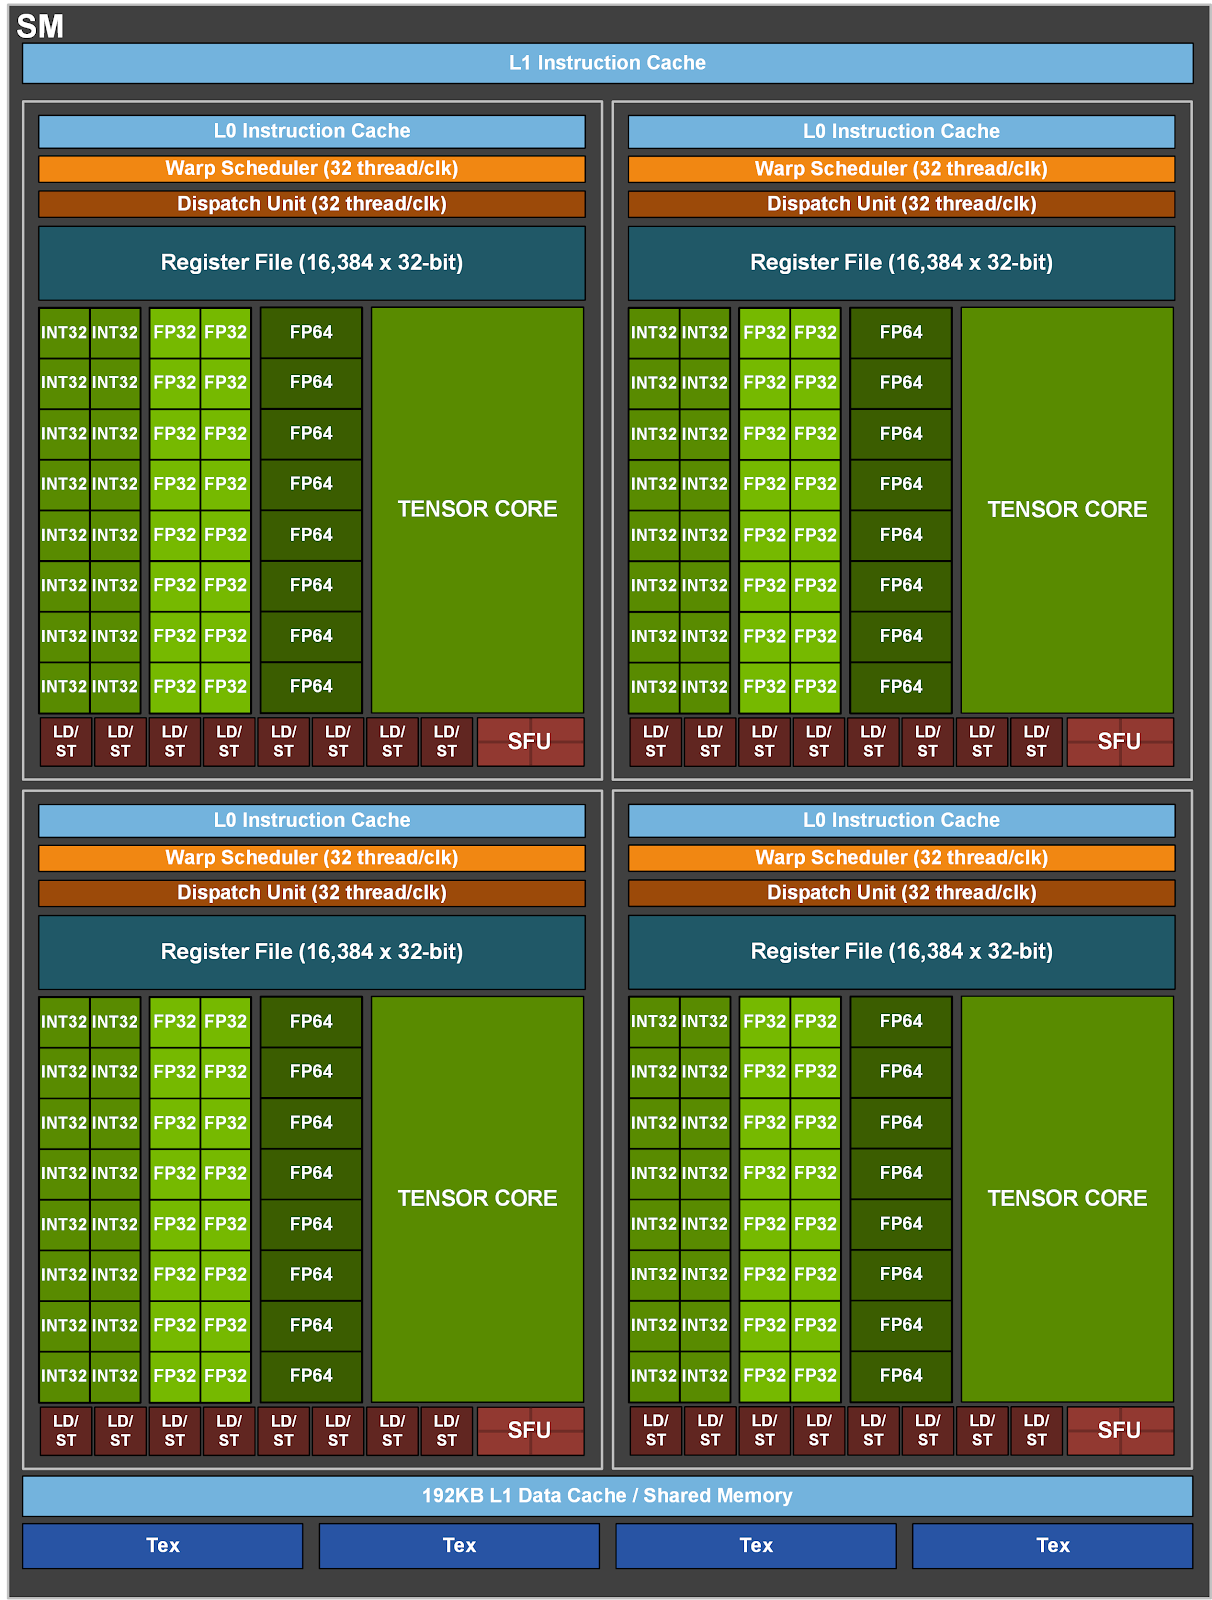
\includegraphics[width=.7\textwidth]{img/a100.png}
    \caption[Diagram of a single A100 SM]{A single SM of an A100 GPU.\\Taken from an NVIDIA Blog Post\footnotemark}
    \label{fig:cuda-sm}
\end{figure}
\footnotetext{\url{https://developer.nvidia.com/blog/nvidia-ampere-architecture-in-depth/}}

based on \cite{mendez2010parallel} and \cite{mendez2012gpu}

\blindtext[3]
\begin{center}
\begin{bytefield}{24}
    \memsection{ffff ffff}{0040 0000}{15}{-- free --}\\
    \begin{rightwordgroup}{internal memory}
        \memsection{003f ffff}{002f c000}{4}{Special Function Registers}\\
        \memsection{002f bfff}{0007 0000}{3}{-- reserved --}\\
        \memsection{0006 ffff}{0000 0000}{8}{Internal Flash}
    \end{rightwordgroup}\\
\end{bytefield}
\end{center}

\begin{center}
    \begin{bytefield}{32}
        \bitheader{0-31} \\
        \bitbox{4}{Four} & \bitbox{8}{Eight} &
        \bitbox{16}{Sixteen} & \bitbox{4}{Four}
    \end{bytefield}
\end{center}
\blindtext[1]
\begin{center}
    \definecolor{lightcyan}{rgb}{0.84,1,1}
    \definecolor{lightgreen}{rgb}{0.64,1,0.71}
    \definecolor{lightred}{rgb}{1,0.7,0.71}
    \begin{bytefield}[bitheight=\widthof{~Base~},
            boxformatting={\centering\small},rightcurly=., rightcurlyspace=0pt]{32}
        % \bitlabel{29}{Data} & \bitlabel{1}{Base} & \bitlabel{2}{Next} \\
        \bitheader{0,28,29,30,31} \\
        \begin{rightwordgroup}{
                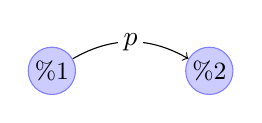
\begin{tikzpicture}
                    \tikzstyle{node}=[circle, draw=blue!50, fill=blue!20, inner sep=1pt, minimum size=6mm]
                    \tikzstyle{linenode}=[pos=0.5,fill=white,inner sep=2pt,outer sep=2pt]
                    \node[node] (A) at (0,0) {\small$\%1$};
                    \node[node] (B) at (2,0) {\small$\%2$};
                    \path [->] (A) edge[bend left] node[linenode] {$p$} (B);
                \end{tikzpicture}
            }
            \bitbox{29}[bgcolor=lightred]{Data} &
            \bitbox{1}[bgcolor=lightcyan]{\rotatebox{90}{Base}} &
            \bitbox{2}[bgcolor=lightgreen]{\rotatebox{90}{Next}}
        \end{rightwordgroup}
    \end{bytefield}
\end{center}
\begin{center}
    \definecolor{lightcyan}{rgb}{0.84,1,1}
    \definecolor{lightgreen}{rgb}{0.64,1,0.71}
    \definecolor{lightred}{rgb}{1,0.7,0.71}
    \begin{bytefield}[bitheight=\widthof{~Base~},
            boxformatting={\centering\small},rightcurly=., rightcurlyspace=0pt, bitwidth=11pt]{32}
        \bitheader{0-31} \\
        \begin{rightwordgroup}{Words}
            \bitbox{29}[bgcolor=lightred]{Data} &
            \bitbox{1}[bgcolor=lightcyan]{\rotatebox{90}{Base}} &
            \bitbox{2}[bgcolor=lightgreen]{\rotatebox{90}{Next}}
        \end{rightwordgroup}
    \end{bytefield}
\end{center}
\blindtext[1]

\subsection{Sparse Bitvectors}
\subsection{Memory Layout}
\subsubsection{Unified Memory}
\subsubsection{64bit Addresses}
\subsection{Concurrent Graph Rewriting}
\subsection{Integration with SVF}
\subsubsection{Parallelizing SVF}
\section{Experimental Results}
\subsection{Test Suite}
\subsection{Bemchmark Suite}
\section{Evaluation}
